\documentclass[10pt]{article}
\usepackage[pdftex]{graphicx}
\usepackage{url}
\usepackage{listings}
\usepackage{pgf}
\usepackage{hyperref}
\usepackage{verbatim}
\usepackage{paralist}
\usepackage{color}

%For plots
\usepackage{pgfplots}

%\usepackage{algpseudocode} %for using the algorithmicx package

\usepackage[lined,boxed,resetcount,longend]{algorithm2e}

\usepackage{proof}
\usepackage{amsmath,amsthm,amssymb}

\newcommand\amp{\mathop{\&}}

\newcommand\pimp{\mathop{\supset}}
\newcommand\pand{\mathop{\wedge}}
\newcommand\por{\mathop{\vee}}
\newcommand\ptrue{\top}
\newcommand\pfalse{\bot}
\newcommand\peq{\Leftrightarrow}

\newcommand\true{\;\textit{true}}
\newcommand\ddd{\raisebox{0.2em}[1.3em]{$\vdots$}}
\newcommand\com{\raisebox{0.3em}{$\ ,\ \ $}}
\newcommand\hyp[2]{\infer[#1]{#2}{}}

\newcommand{\DD}{\mathcal{D}}
\newcommand{\EE}{\mathcal{E}}
\newcommand{\FF}{\mathcal{F}}

\newcommand{\COPY}{\text{\textbf{[COPY]}}}
\newcommand{\LOAD}{\text{\textbf{[LOAD]}}}
\newcommand{\ADDROF}{\text{\textbf{[ADDROF]}}}
\newcommand{\STORE}{\text{\textbf{[STORE]}}}
\newcommand{\CALL}{\text{\textbf{[CALL]}}}

\newcommand{\set}[1]{\{#1\}}

\newcommand{\pointsto}[2]{\mathcal{P}_{[#1]}(#2)}

%for algorithm2e -within figure
\renewcommand\topfraction{0.85}
\renewcommand\bottomfraction{0.85}
\renewcommand\textfraction{0.1}
\renewcommand\floatpagefraction{0.85}

\newcommand{\myvar}[1]{\texttt{\$#1}}

\newcommand{\EmbedCode}[3]{
	\lstset{language=#1}
	\lstset{backgroundcolor=\color{white},rulecolor=}
	\lstset{linewidth=\textwidth}
	\lstset{commentstyle=\textit, stringstyle=\upshape,showspaces=false}
	\lstset{frame=shadowbox,
			showstringspaces=false,
			numbers=#3,
			numberblanklines=false}
	\lstinputlisting[]{#2} 
}

\newcommand{\main}{\texttt{main}}
\newcommand{\even}{\texttt{even}}
\newcommand{\odd}{\texttt{odd}}
\newcommand{\compute}{\texttt{compute}}

\topmargin -0.1pt
\advance \topmargin by -\headheight
\advance \topmargin by -\headsep
\textheight 9.2in
\oddsidemargin -0.1pt
\evensidemargin \oddsidemargin
\marginparwidth 1in
\textwidth 6.3in

\parindent 0in
\parskip 1.5ex

\title{Static Analysis for Software Engineering\\
		Midterm Report \\
		Project: Static Taint Analysis for C}
\author{Xavier Noumbissi}
\date{}

\lstset{ %
language=c,
basicstyle=\scriptsize,commentstyle=\scriptsize\itshape,showstringspaces=false,breaklines=true}


\begin{document}
\maketitle

\section{Introduction}

We proposed to develop a static taint analysis in our
project proposal.
This paper presents the design of our taint analysis.
We first present a motivating example in Section~\ref{example},
then explain in Section~\ref{sec:sampleSummary} how our analysis
would perform on the example. We finally give a detailed
description of our analysis in Section~\ref{analysis}.

\subsection{Motivating Example}\label{example} 

\begin{figure}[!h]
\begin{center}
\EmbedCode{c}{main.c}{left}
\end{center}
\caption{Motivating Example}
\label{fig:sample}
\end{figure}

Figure~\ref{fig:sample} shows $4$ C functions:
\main, \even, \odd, and \compute.

In \main{}, function \texttt{scanf} from the standard input/ouput
library gets an integer input from user at line $3$
and stores it in variable \texttt{x}. \texttt{x} 
becomes \textit{tainted} since it holds a value from
the environment which has not been validated and
sanitized.
\texttt{x} is later used in line $4$ as argument to \even{}
and at line $6$ as argument to \odd{}.

In \compute{}, variable \texttt{sum} gets tainted at
line $13$ through function \texttt{scanf}. Variable
\texttt{x} is tainted only if it was passed tainted
at calling sites.

In functions \even{}, and \odd{}, variable \texttt{x}
is tainted only when it has been passed as tainted
at calling sites.

\begin{comment}
\begin{figure}
\begin{minipage}[b]{0.45\textwidth}
	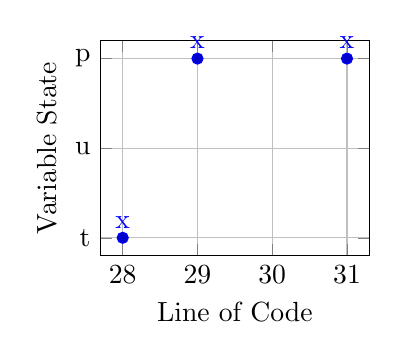
\begin{tikzpicture}
		\begin{axis}[
					 xlabel=Line of Code,					 
					 symbolic y coords={t,u,p},		
					 ylabel=Variable State,				
					 ytick={t,u,p},
					 xtick={28,29, ...,31},
					 grid=both,
					 width=5cm				 
					 ]				 
			\addplot+ [only marks,
					   nodes near coords=x ] coordinates {
				(28,t)
				(29,p)
				(31,p)
				};
		\end{axis}
	\end{tikzpicture}	
	\caption{Taint Information for \main{}}\label{fig:taintmain}
	\end{minipage}		
	\begin{minipage}[b]{0.45\textwidth}
	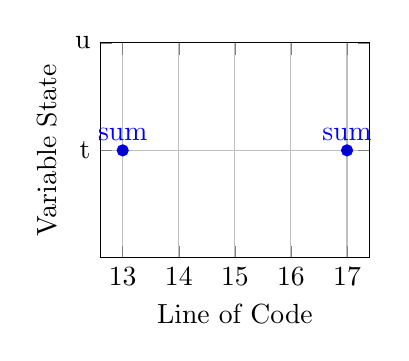
\begin{tikzpicture}
		\begin{axis}[
					 xlabel=Line of Code,					 
					 symbolic y coords={t,u,p},		
					 ylabel=Variable State,				
					 ytick={t,u,p},
					 xtick={11,12, ...,18},
					 grid=both,
					 width=5cm				 
					 ]				 
			\addplot+ [only marks,
					   nodes near coords=sum ] coordinates {
				(13,t)
				(17,t)				
				};
		\end{axis}
	\end{tikzpicture}	
	\caption{Taint Information for \compute{}}\label{fig:taintcompute}
	\end{minipage}			
\end{figure}
\end{comment}

\subsection{Handling of complex data structures}


\section{Analysis}\label{analysis}


\bibliographystyle{plain}
\bibliography{mr}

\end{document}









